\documentclass[a4paper,10pt,twoside]{article}

\usepackage[top=1in, bottom=1in, left=1in, right=1in]{geometry}
\usepackage[utf8]{inputenc}
\usepackage[spanish,es-ucroman,es-noquoting]{babel}
\usepackage{setspace}
\usepackage{fancyhdr}
\usepackage{lastpage}
\usepackage{amsmath}
\usepackage{amsfonts}
\usepackage{verbatim}
\usepackage{listings}
\usepackage{graphicx}
\usepackage{float}
\usepackage{algorithmic}
\usepackage{color}
\usepackage{hyperref}
\usepackage[usenames,dvipsnames]{xcolor}
\definecolor{dkgreen}{rgb}{0,0.6,0}
\definecolor{gray}{rgb}{0.97,0.97,0.97}
\definecolor{mauve}{rgb}{0.58,0,0.82}
\usepackage{tikz}
\usetikzlibrary{calc}
\usetikzlibrary{decorations.pathreplacing}
\usepackage{ragged2e}

\lstset{
    backgroundcolor=\color{lbcolor},
    tabsize=4,
    rulecolor=,
    language=matlab,
        basicstyle=\scriptsize,
        upquote=true,
        aboveskip={1.5\baselineskip},
        columns=fixed,
        showstringspaces=false,
        extendedchars=true,
        breaklines=true,
        prebreak = \raisebox{0ex}[0ex][0ex]{\ensuremath{\hookleftarrow}},
        frame=single,
        showtabs=false,
        showspaces=false,
        showstringspaces=false,
        identifierstyle=\ttfamily,
        keywordstyle=\color[rgb]{0,0,1},
        commentstyle=\color[rgb]{0.133,0.545,0.133},
        stringstyle=\color[rgb]{0.627,0.126,0.941},
}

% Evita que el documento se estire verticalmente para ocupar
% el espacio vacío en cada página.
\raggedbottom


%%%%%%%%%% Configuración de Fancyhdr - Inicio %%%%%%%%%%
\pagestyle{fancy}
\thispagestyle{fancy}
\lhead{Trabajo Práctico 3, Organización del Computador II}
\rhead{Chapresto, Rey, Vileriño}
\renewcommand{\footrulewidth}{0.4pt}
\cfoot{\thepage /\pageref{LastPage}}

\fancypagestyle{caratula} {
   \fancyhf{}
   \cfoot{\thepage /\pageref{LastPage}}
   \renewcommand{\headrulewidth}{0pt}
   \renewcommand{\footrulewidth}{0pt}
}
%%%%%%%%%% Configuración de Fancyhdr - Fin %%%%%%%%%%


%%%%%%%%%% Configuración de Algorithmic - Inicio %%%%%%%%%%
% Entorno propio para customizar la presentación del pseudocódigo
\newenvironment{pseudocodigo}
    {\vspace{0.5em} \begin{algorithmic}}
    {\end{algorithmic} \vspace{0.5em}}

% Alinear comentarios a la derecha
\renewcommand{\algorithmiccomment}[1]{\hfill \{#1\}}
%%%%%%%%%% Configuración de Algorithmic - Fin %%%%%%%%%%


%%%%%%%%%% Macros de tikz - Inicio %%%%%%%%%%
% Uso: \registroCuatro{etiqueta}{x}{y}{a4}{a3}{a2}{a1}
\newcommand{\registroCuatro}[7]{
    \ifthenelse{\equal{#1}{}}{}{
        \draw (#2, {#3 + 0.5}) node[anchor=east]{#1};
    }

    \draw   (#2, #3) rectangle +(4, 1) +(2, 0.5) node{#4}
          ++(4, 0)   rectangle +(4, 1) +(2, 0.5) node{#5}
          ++(4, 0)   rectangle +(4, 1) +(2, 0.5) node{#6}
          ++(4, 0)   rectangle +(4, 1) +(2, 0.5) node{#7};          
}

% Uso: \registroOcho{etiqueta}{x}{y}{a8}{a7}{a6}...{a1}
\newcommand{\registroOcho}[9]{
    \def\etiqueta{#1}
    \def\x{#2}
    \def\y{#3}
    \def\aviii{#4}
    \def\avii{#5}
    \def\avi{#6}
    \def\av{#7}
    \def\aiv{#8}
    \def\aiii{#9}
    \registroOchoX    
}
\newcommand{\registroOchoX}[2]{ % Auxiliar - no usar directamente
    \def\aii{#1}
    \def\ai{#2}
    \ifthenelse{\equal{\etiqueta}{}}{}{
        \draw (\x, {\y + 0.5}) node[anchor=east]{\etiqueta};
    }
    \filldraw[fill=white]
        (\x, \y) rectangle +(2, 1) +(1, 0.5) node{\aviii}
        ++(2, 0) rectangle +(2, 1) +(1, 0.5) node{\avii}
        ++(2, 0) rectangle +(2, 1) +(1, 0.5) node{\avi}
        ++(2, 0) rectangle +(2, 1) +(1, 0.5) node{\av}
        ++(2, 0) rectangle +(2, 1) +(1, 0.5) node{\aiv}
        ++(2, 0) rectangle +(2, 1) +(1, 0.5) node{\aiii}
        ++(2, 0) rectangle +(2, 1) +(1, 0.5) node{\aii}
        ++(2, 0) rectangle +(2, 1) +(1, 0.5) node{\ai};
}


% Uso: \registroDieciseis{etiqueta}{x}{y}{a16}{a15}{a14}...{a1}
\newcommand{\registroDieciseis}[9]{
    \def\etiqueta{#1}
    \def\x{#2}
    \def\y{#3}
    \def\axvi{#4}
    \def\axv{#5}
    \def\axiv{#6}
    \def\axiii{#7}
    \def\axii{#8}
    \def\axi{#9}
    \registroDieciseisX
}
\newcommand{\registroDieciseisX}[9]{ % Auxiliar - no usar directamente
    \def\ax{#1}
    \def\aix{#2}
    \def\aviii{#3}
    \def\avii{#4}
    \def\avi{#5}
    \def\av{#6}
    \def\aiv{#7}
    \def\aiii{#8}
    \def\aii{#9}
    \registroDieciseisXX
}
\newcommand{\registroDieciseisXX}[1]{ % Auxiliar - no usar directamente
    \def\ai{#1}
    \ifthenelse{\equal{\etiqueta}{}}{}{
        \draw (\x, {\y + 0.5}) node[anchor=east]{\etiqueta};
    }
    \filldraw[fill=white]
        (\x, \y) rectangle +(1, 1) +(0.5, 0.5) node{\axvi}
        ++(1, 0) rectangle +(1, 1) +(0.5, 0.5) node{\axv}
        ++(1, 0) rectangle +(1, 1) +(0.5, 0.5) node{\axiv}
        ++(1, 0) rectangle +(1, 1) +(0.5, 0.5) node{\axiii}
        ++(1, 0) rectangle +(1, 1) +(0.5, 0.5) node{\axii}
        ++(1, 0) rectangle +(1, 1) +(0.5, 0.5) node{\axi}
        ++(1, 0) rectangle +(1, 1) +(0.5, 0.5) node{\ax}
        ++(1, 0) rectangle +(1, 1) +(0.5, 0.5) node{\aix}
        ++(1, 0) rectangle +(1, 1) +(0.5, 0.5) node{\aviii}
        ++(1, 0) rectangle +(1, 1) +(0.5, 0.5) node{\avii}
        ++(1, 0) rectangle +(1, 1) +(0.5, 0.5) node{\avi}
        ++(1, 0) rectangle +(1, 1) +(0.5, 0.5) node{\av}
        ++(1, 0) rectangle +(1, 1) +(0.5, 0.5) node{\aiv}
        ++(1, 0) rectangle +(1, 1) +(0.5, 0.5) node{\aiii}
        ++(1, 0) rectangle +(1, 1) +(0.5, 0.5) node{\aii}
        ++(1, 0) rectangle +(1, 1) +(0.5, 0.5) node{\ai};
}
%%%%%%%%%% Macros de tikz - Fin %%%%%%%%%%


%%%%%%%%%% Macros misceláneos - Inicio %%%%%%%%%%
\newcommand{\xmm}[1]{\texttt{XMM#1}}
\newcommand{\rax}{\texttt{RAX}}
\newcommand{\rbx}{\texttt{RBX}}
\newcommand{\rcx}{\texttt{RCX}}
\newcommand{\rdx}{\texttt{RDX}}
\newcommand{\rbp}{\texttt{RBP}}
\newcommand{\rsp}{\texttt{RSP}}
\newcommand{\reg}[1]{\texttt{R#1}}
\newcommand{\asm}[1]{\texttt{\uppercase{#1}}}
%%%%%%%%%% Macros misceláneos - Fin %%%%%%%%%%


\begin{document}


%%%%%%%%%%%%%%%%%%%%%%%%%%%%%%%%%%%%%%%%%%%%%%%%%%%%%%%%%%%%%%%%%%%%%%%%%%%%%%%
%% Carátula                                                                  %%
%%%%%%%%%%%%%%%%%%%%%%%%%%%%%%%%%%%%%%%%%%%%%%%%%%%%%%%%%%%%%%%%%%%%%%%%%%%%%%%


\thispagestyle{caratula}

\begin{center}


\includegraphics[height=2cm]{DC.png} 
\hfill

\includegraphics[height=2cm]{UBA.jpg} 

\vspace{2cm}

Departamento de Computación,\\
Facultad de Ciencias Exactas y Naturales,\\
Universidad de Buenos Aires

\vspace{4cm}

\begin{Huge}
Trabajo Práctico 3
\end{Huge}

\vspace{0.5cm}

\begin{Large}
Organización del Computador II
\end{Large}

\vspace{1cm}

Segundo Cuatrimestre de 2013

\vspace{4cm}

Grupo: \textbf{Crema Americana/Persico}

\vspace{0.5cm}

\begin{tabular}{|c|c|c|}
    \hline
    Apellido y Nombre & LU & E-mail\\
    \hline
    Silvio Vileriño             & 106/12 & svilerino@gmail.com\\
    Esteban Rey 				& 657/10 & estebanlucianorey@gmail.com\\
    Matias Chapresto 			& 201/12 & matiaschapresto@gmail.com\\
    \hline
\end{tabular}

\vspace{1cm}


\end{center}
\newpage


%%%%%%%%%%%%%%%%%%%%%%%%%%%%%%%%%%%%%%%%%%%%%%%%%%%%%%%%%%%%%%%%%%%%%%%%%%%%%%%
%% Índice                                                                    %%
%%%%%%%%%%%%%%%%%%%%%%%%%%%%%%%%%%%%%%%%%%%%%%%%%%%%%%%%%%%%%%%%%%%%%%%%%%%%%%%


\tableofcontents

\newpage



%%%%%%%%%%%%%%%%%%%%%%%%%%%%%%%%%%%%%%%%%%%%%%%%%%%%%%%%%%%%%%%%%%%%%%%%%%%%%%%
%% Introduccion                                                              %%
%%%%%%%%%%%%%%%%%%%%%%%%%%%%%%%%%%%%%%%%%%%%%%%%%%%%%%%%%%%%%%%%%%%%%%%%%%%%%%%


\section{Introduccion}

En el siguiente informe se describen las caracteristicas del TP entregado. Se separo en secciones con similitud a la secuencia de enunciados provistos por la catedra mas una seccion "Modularizacion de codigo" que indica como fue organizado el desarrollo por el grupo. La seccion "Interfaz con el usuario" describe el manejo de las pantallas mapa y estado y su interaccion con los demas modulos.\\

Para la realizacion del TP, al darse los temas para su desarrollo de forma gradual, quedo separado en distintas etapas: Pasaje a modo protegido configurando la GDT,  establecimiento del sistema de paginacion, habilitacion las interrupciones, inicializacion de tareas y organizacion del scheduller. A todo esto se le suma la interfaz grafica, la cual requeria consumir de los datos obtenidos de las demas etapas. Como el desarrollo implico tocar constantemente todas las partes, decidimos escribir de la misma forma el informe, con excepcion de la interfaz grafica.


%%%%%%%%%%%%%%%%%%%%%%%%%%%%%%%%%%%%%%%%%%%%%%%%%%%%%%%%%%%%%%%%%%%%%%%%%%%%%%%
%% Desarrollo                                                                %%
%%%%%%%%%%%%%%%%%%%%%%%%%%%%%%%%%%%%%%%%%%%%%%%%%%%%%%%%%%%%%%%%%%%%%%%%%%%%%%%


\section{Desarrollo}

\subsection{Modularizacion del codigo}

Como el codigo fue creciendo de a poco, notamos que, de equivocarnos en una seccion que era utilizada por otras, implicaba tocar todos los documentos una y otra vez, para resolver el error. Para solucionar esto optamos por aislar de alguna forma las secciones con una capa intermedia, la cual guardaria toda la informacion necesaria para el sistema y la expondria a cada seccion, solo el tipo de datos necesario. Por ejemplo, como tenemos 3 tipos de direcciones:fisica, virtual y de pantalla, centramos todas las conversiones entre estas tres en un modulo que llamamos "Context Manager" y cada seccion solo recibe el tipo de direccion que requiere, sin tener que incluir en el codigo las conversiones.\\

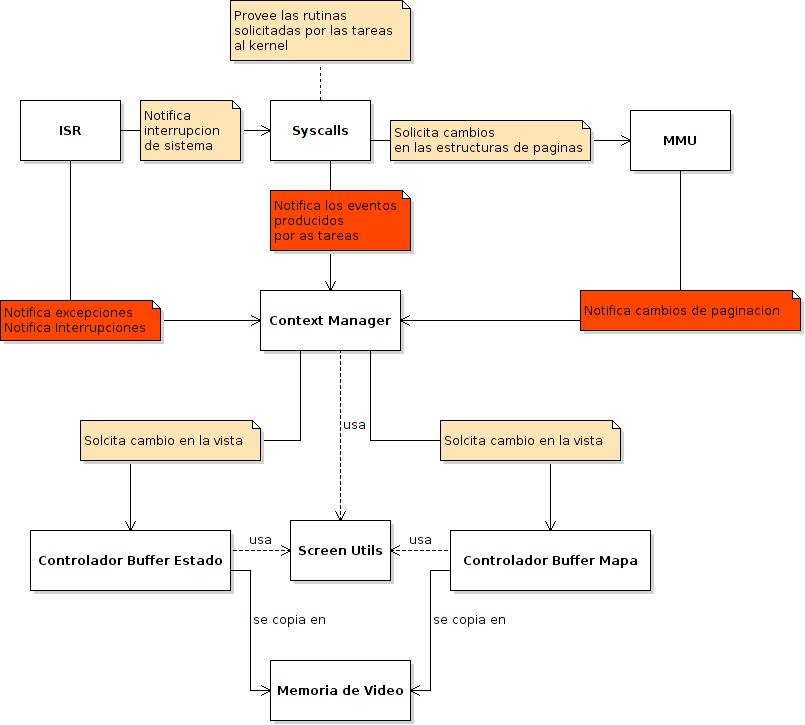
\includegraphics[scale=0.5]{diagramas/contextManager-relaciones.jpg}   
\\Context Manager y sus relaciones con las demas secciones. Imagen sin especificar las funciones internas\\

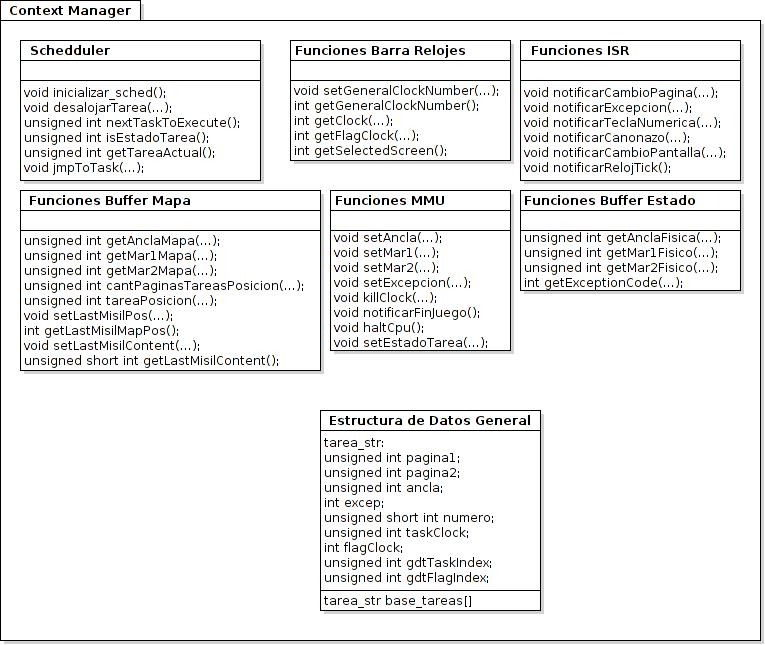
\includegraphics[scale=0.5]{diagramas/contextManager.jpg}   
\\Funciones y estructuras del Context Manager\\


Siendo de esta forma un paso intermedio entre las partes, la secuencia de accion de cada funcionalidad del juego pasa por el mismo. En las siguientes secciones se mostrara como las distintas funcionalidades utilizan esta estructura.

\newpage

\subsection{Inicializacion y Segmentacion}

Para iniciar el sistema se paso de modo real a modo protegido, para ello necesitamos establecer una GDT que nos delimite los distintos segmentos a usar por nuestro kernel.\\

Por enunciado se pedian 5 descriptores, 1 de video, codigo de nivel kernel, datos de nivel kernel, codigo de nivel usuario y datos de nivel usuario. Se definio por cada entrada un indice (en orden del 18 al 22) y un descriptor:

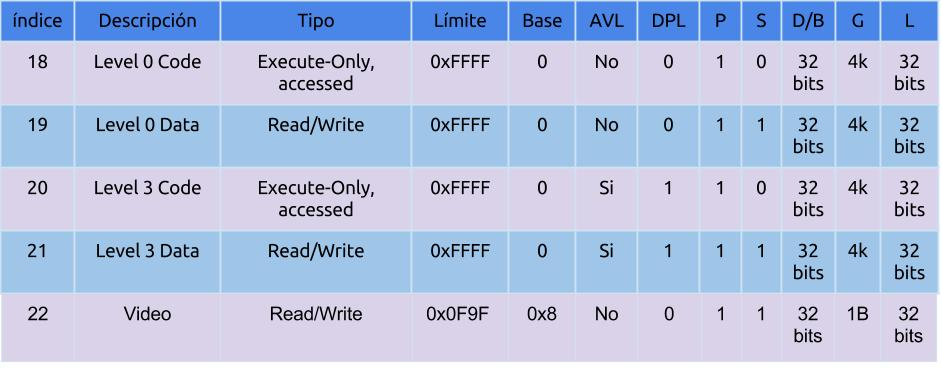
\includegraphics[scale=0.4]{diagramas/gdt-primerasEntradas.jpg} 
\\Organizacion de la GDT: primeras entradas.\\

Una vez completa, se incluyo en el codigo del kernel la instruccion LGDT para cargar en el procesador la direccion de memoria de la misma. Paso seguido seteamos el bit 0 del registro CR0 en 1 para pasar al modo protegido y efectuamos un salto para hacer que el procesador se setee en el segmento de codigo de kernel, indice 18 de la GDT con la instruccion JMP 0x90:protected$\_$mode. Se utiliza el valor 0x90 para saltar al segmento correspondiente ya que el indice del segmento al que necesitamos ir (codigo de kernel) es el 18$_10$. Como el RPL es 0 de kernel y estoy accediendo a una entrada de la GDT, los 3 primeros bits del selector son 0, equivalente de multiplicar por 8: 18$_10$ x 8$_10$ = 0x90

Despues seteamos los registros selectores a los segmentos correspondientes e inicializamos la pila del kernel en la posicion 0x27000, pasandole este valor al registro ESP y EBP.



\lstinputlisting[tabsize=4, numbers=left, numberstyle=\tiny\color{black},mathescape=true, backgroundcolor=\color{gray}, rulecolor=\color{black}, keywordstyle=\color{blue}, commentstyle=\color{dkgreen},stringstyle=\color{mauve}, numbersep=5pt, basicstyle=\scriptsize]{diagramas/kernel.asm}

\newpage
\subsection{Descriptor de Interrupciones y Handlers}
Previo a cualquier configuracion o funcion a llamar dentro de nuestro kernel, se llamo a la instruccion CLI, la cual nos deshabilito las interrupciones ("saltando a modo protegido"). Una vez deshabilitadas y en modo protegido, establecimos la tabla de interrupciones con la instruccion LIDT. A esta instruccion le pasamos la tabla ya configurada, con las interrupciones posibles: tanto las excepciones como las interrupciones. Cada entrada fue configurada para ser ejecutada en el segmento de codigo de kernel (selector 0x90), ya que el debe ser el responsable de ellas. Las rutinas de atencion, configuradas en el offset de cada descriptor de la IDT, notifican al context manager el evento producido, para que este actualice los datos en los distintos modulos: sea pantalla o mmu. 

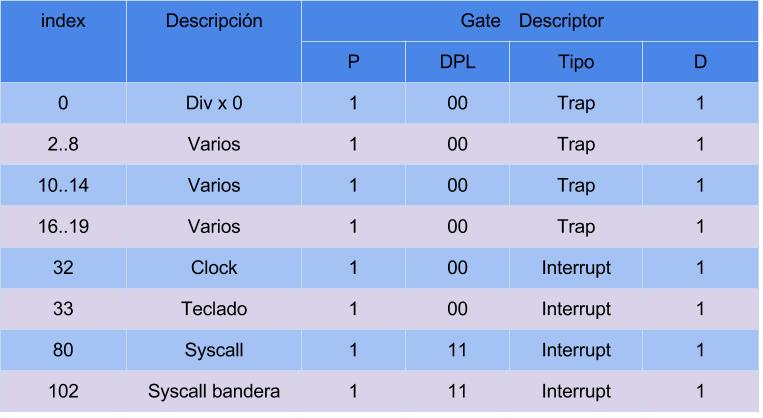
\includegraphics[scale=0.4]{diagramas/idt.jpg}
\\Descriptores de la IDT.\\

Los campos de offset se completaron con la direccion de los handlers de atencion a las interrupciones, en donde dependiendo del tipo, se recurre a distintos modulos para resolver el evento producido.\\

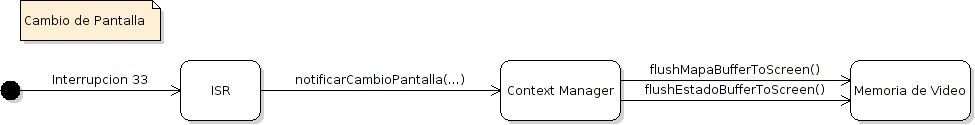
\includegraphics[scale=0.4]{diagramas/cambioPantalla-handler.jpg}
\\\centering{Manejador de cambio de pantalla}\\
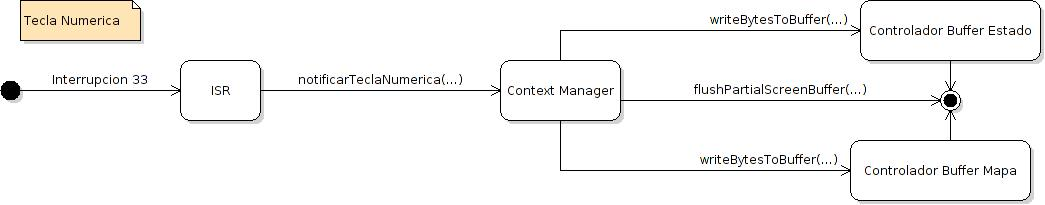
\includegraphics[scale=0.4]{diagramas/teclaNumerica-handler.jpg}
\\\centering{Interrupcion por tecla num\'erica}\\
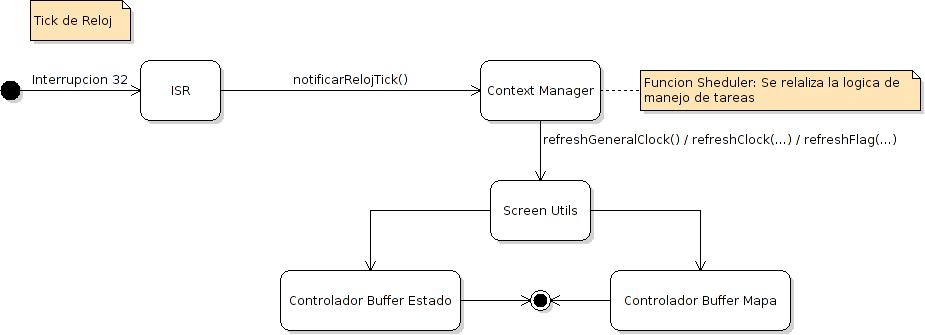
\includegraphics[scale=0.4]{diagramas/tickReloj-handler.jpg}
\\\centering{Interrupcion del clock}\\
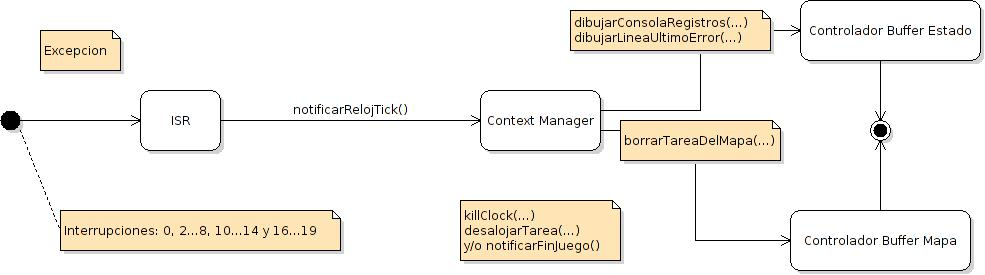
\includegraphics[scale=0.4]{diagramas/excepcion-handler.jpg}
\\\centering{Manejo de las excepci\'ones}\\
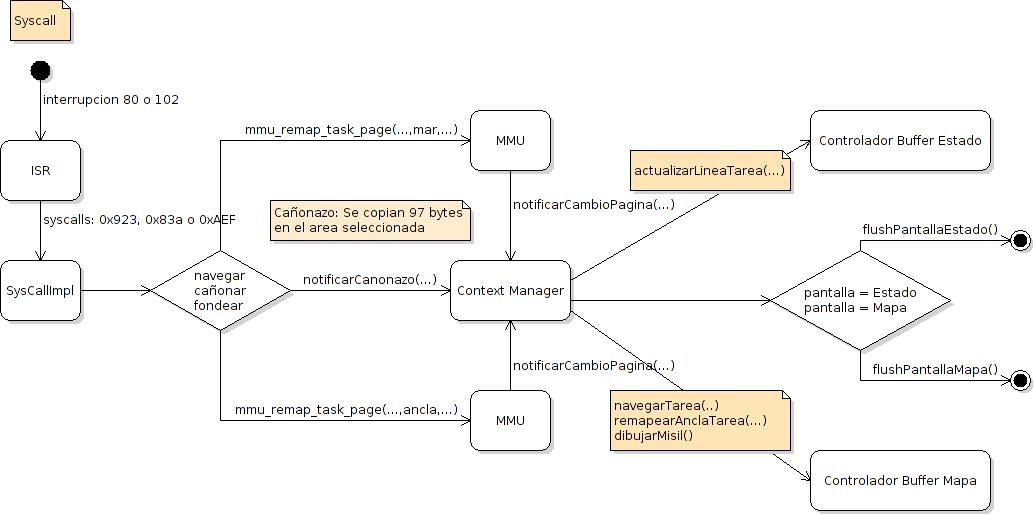
\includegraphics[scale=0.4]{diagramas/syscall-handler.jpg}
\\\centering{Llamadas al sistema}\\




\newpage
\subsection{Paginacion}

\justifying
Para activar la paginacion es necesario que armemos el sistema de directorios y paginas del kernel. Como se requirio un identity mapping para el kernel, de los primeros 7.5Mb de memoria, utilizamos entradas en el directorio. La primer entrada posee todas las posiciones de la tabla inicializadas en Present, marcando asi los primeros 4Mb. La segunda entrada, sin embargo solo debe mapear 3.5Mb, con lo cual solo se necesitan 896 entradas mas marcadas como presentes.\\

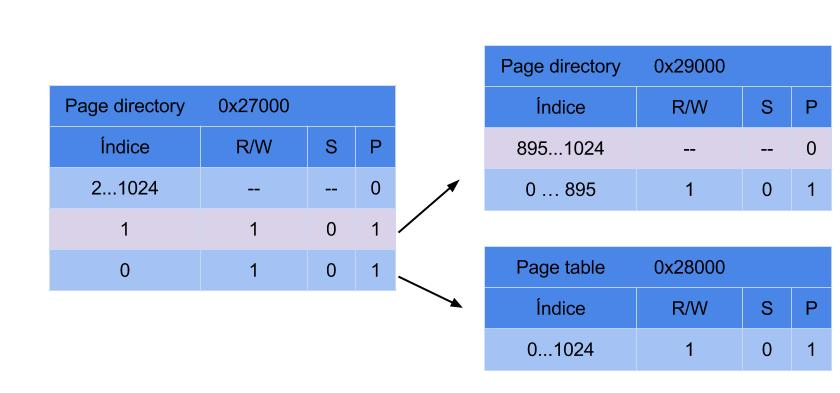
\includegraphics[scale=0.4]{diagramas/paginacionKernel.jpg}
\\\centering{Distribucion de paginas del kernel y posicion de los directorios.}\\
\justifying
Para el paginado de las tareas se requerian por enunciado 3 paginas: 2 para la tarea que debian mapearse en el mar (arriba del primer giga) y una tercera, el ancla, que debia apuntar al espacio de memoria del kernel (no modificable). La estructura del directorio y de las tablas se pusieron contiguas a las del kernel, en su area de memoria. Para ubicar las tareas a partir de la direccion virtual 0x40000000, se utilizo el indice 256 de sus directorios y cada tabla apuntando de a 4Mb: 0x40000000, 40001000 y 40002000. Tambien fue necesario inicializar 2 entradas en el directorio de cada tarea con identity mapping a la memoria del kernel, para que este pudiese ejecutarse en el contexto de la tarea. Estas entradas poseen acceso solo por el kernel y permiten la ejecucion de los handlers de interrupciones.

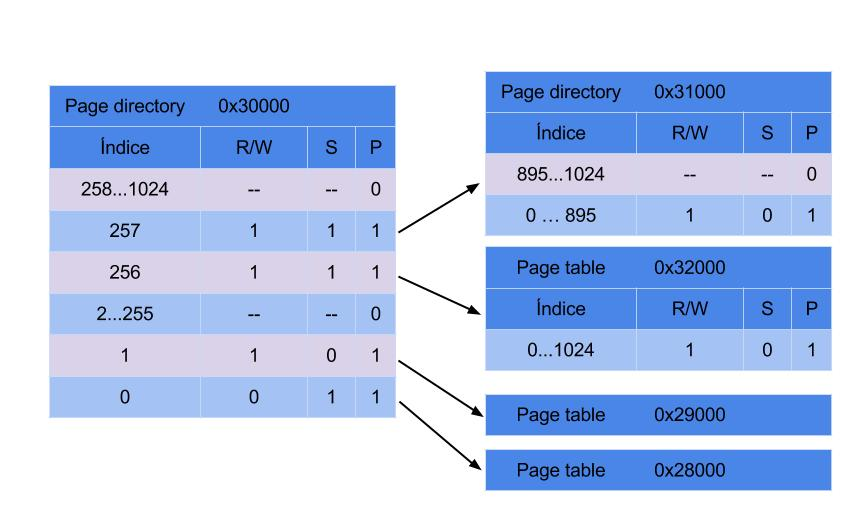
\includegraphics[scale=0.4]{diagramas/paginacionTarea.jpg}
\\\centering{Mapeo generico de una tarea.}\\
\justifying
Como las tareas son capaces de "moverse" se puso a disposicion de la mmu funciones para remapear las paginas propias. Se paso de forma mas directa la informacion soblre las paginas al Context Manager para poder reflejar el movimiento de las paginas en la pantalla del mapa y en los indicadores de la pantalla de estado. 


\newpage
\subsection{Tareas: Descriptores y contexto}

Al saltar por primera vez a la tarea idle, nos aseguramos de tener inicializadas todas las TSS de las distintas tareas (2 por tarea, uno para la tarea en si y la otra para la bandera). La tarea inicial, desde donde se salta por primera vez a la idle, tambien debe tener un espacio pare el contexto de ejecucion, en donde el procesador guardara el estado del kernel para luego pasar a la ejecucion de tareas. La tarea idle debe ser mapeada sobre la memoria del kernel y compartir su CR3; ya que de no ser asi, y ubicarla en el mar con las demas, corremos el riesgo de que sea corrompida por otra tarea mediante un cañonazo, comprometendo la estabilidad del sistema.

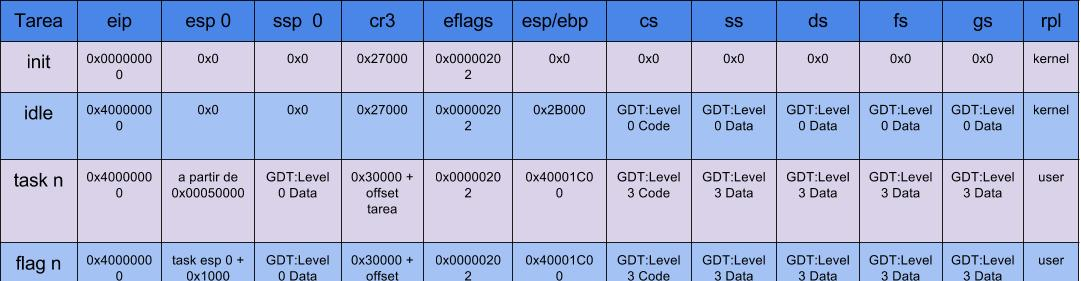
\includegraphics[scale=0.4]{diagramas/descriptoresDeTareas.jpg}
Mapeo en memoria del contexto de ejecucion de la tarea Idle y de las tareas.\\


Para que el procesador ubique la TSS de la tarea, incluimos en la GDT, por cada una, 2 entradas (tarea y bandera). Estas entradas son Descriptores de tarea, y le seteamos el limite minimo para las TSS que es de 0x67.

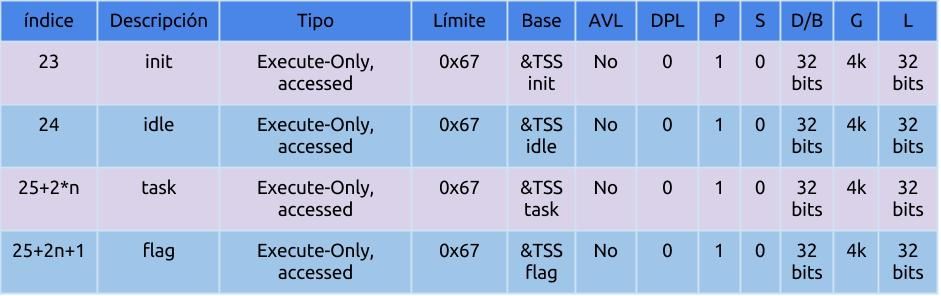
\includegraphics[scale=0.4]{diagramas/entradasGDTParaTareas.jpg}
Valores de las entradas de la GDT para la tarea Idle, Tareas y Banderas.\\




\newpage
\subsection{Interfaz con el usuario}
Las 2 pantallas del sistema muestran todos los datos utilizados por el mismo y los movimientos de las tareas por el mar y sus anclas por la tierra. Esta parte de la funcionalidad del kernel solo conoce sobre posiciones de mapa, caracterizada por la cantidad de memoria de cada buffer de pantalla. La adecuacion de las posiciones se llevan a cabo en el Context Manager, el cual traduce las direcciones fisicas y virtuales en datos para mostrar en los distintos sectores de la pantalla.

Las pantallas tienen en comun 2 secciones: el nombre de grupo en la parte superior, y la barra de relojes en la inferior. El nombre de grupo es seteado permanentemente al inicio del sistema, mientras que, por otro lado, los relojes son actualizados cada vez que una tarea corre.

Todos los elementos dinamicos de las pantallas fuenron pensados para actualizarse por eventos de forma individual, para no tener que copiar todo el buffer de cada pantalla, cada vez que un reloj se movia. Cada sector responde a un evento el cual es delegado a traves del Context Manager a las secciones de manejo de Buffers.


\subsection{Schedduler}

\input{shedduler}


\end{document}